% Convergence of the thousandth eigenvalue against the degrees of freedom,
% L-shaped domain: the eigenvalue itself on the left, the relative error on the
% right.
%
% Requires in the preamble:
%   \usepackage{graphicx}
%   \usepackage{subfig}
%   \usepackage{epstopdf}   % the figures are EPS; needed under pdflatex,
%                           % which then wants -shell-escape. Not needed for
%                           % latex/dvips, which reads EPS directly.
%
% The figures live next to this file, in
% results_paper/eigenvalues_convergence/. If you \input this snippet
% from elsewhere, point graphicx at that folder, e.g.
%   \graphicspath{{results_paper/eigenvalues_convergence/}}
% and drop the leading path from the \includegraphics arguments below.

\begin{figure}[htbp]
  \centering
  \subfloat[Eigenvalue $\lambda_{1000}$.\label{fig:convergence_L_shaped_lambda1000_value}]{%
    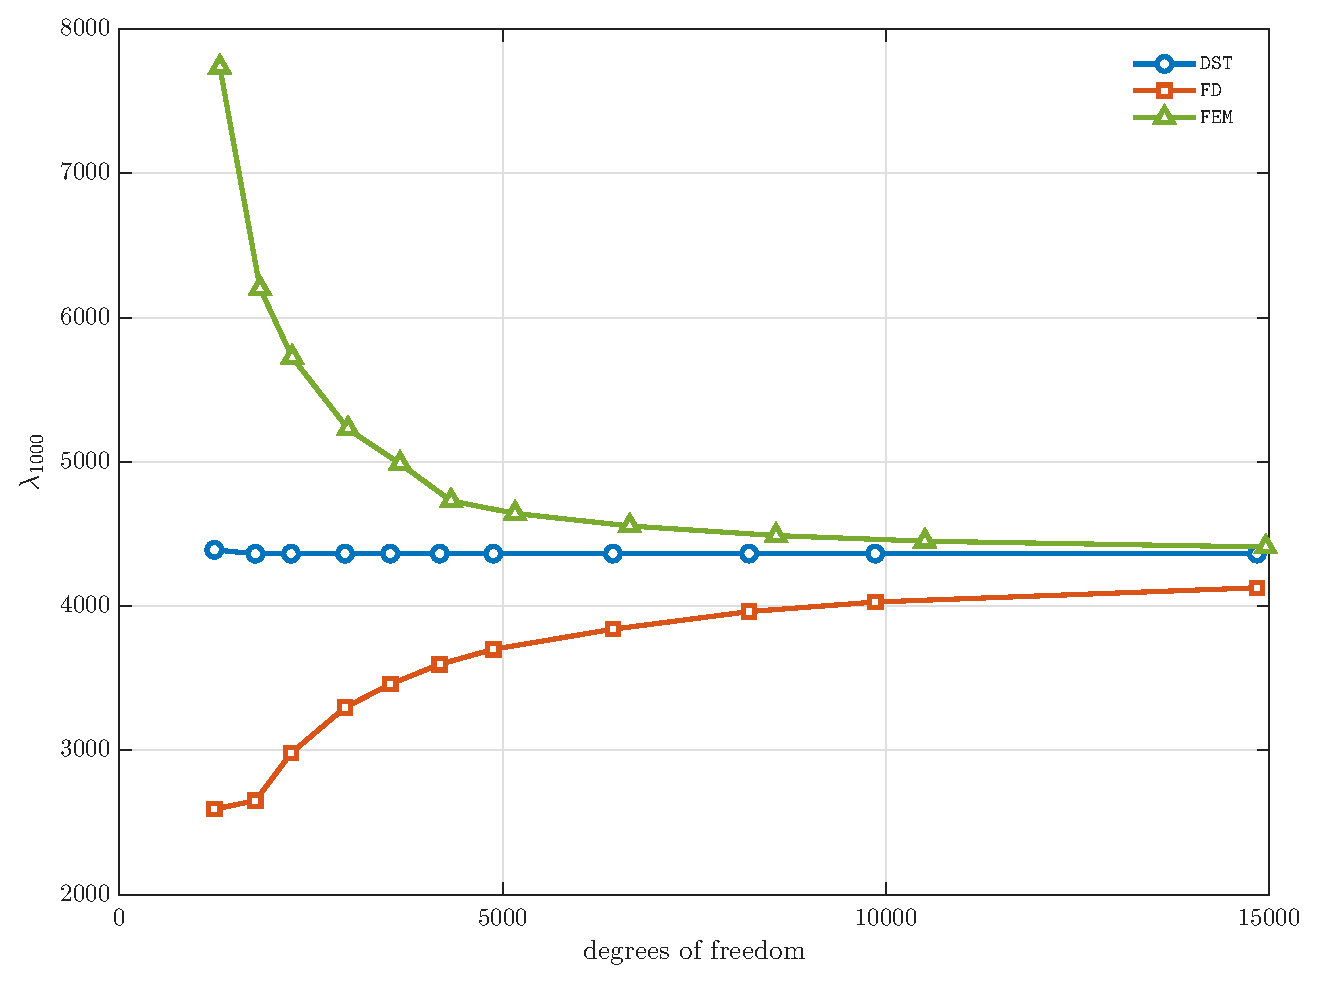
\includegraphics[width=0.45\textwidth]{L_shaped_convergence_lambda1000}}
  \qquad
  \subfloat[Relative error $\frac{|\lambda_{1000} - \lambda_{1000}^{\text{DST}}|}{\lambda_{1000}^{\text{DST}}}$.\label{fig:convergence_L_shaped_lambda1000_error}]{%
    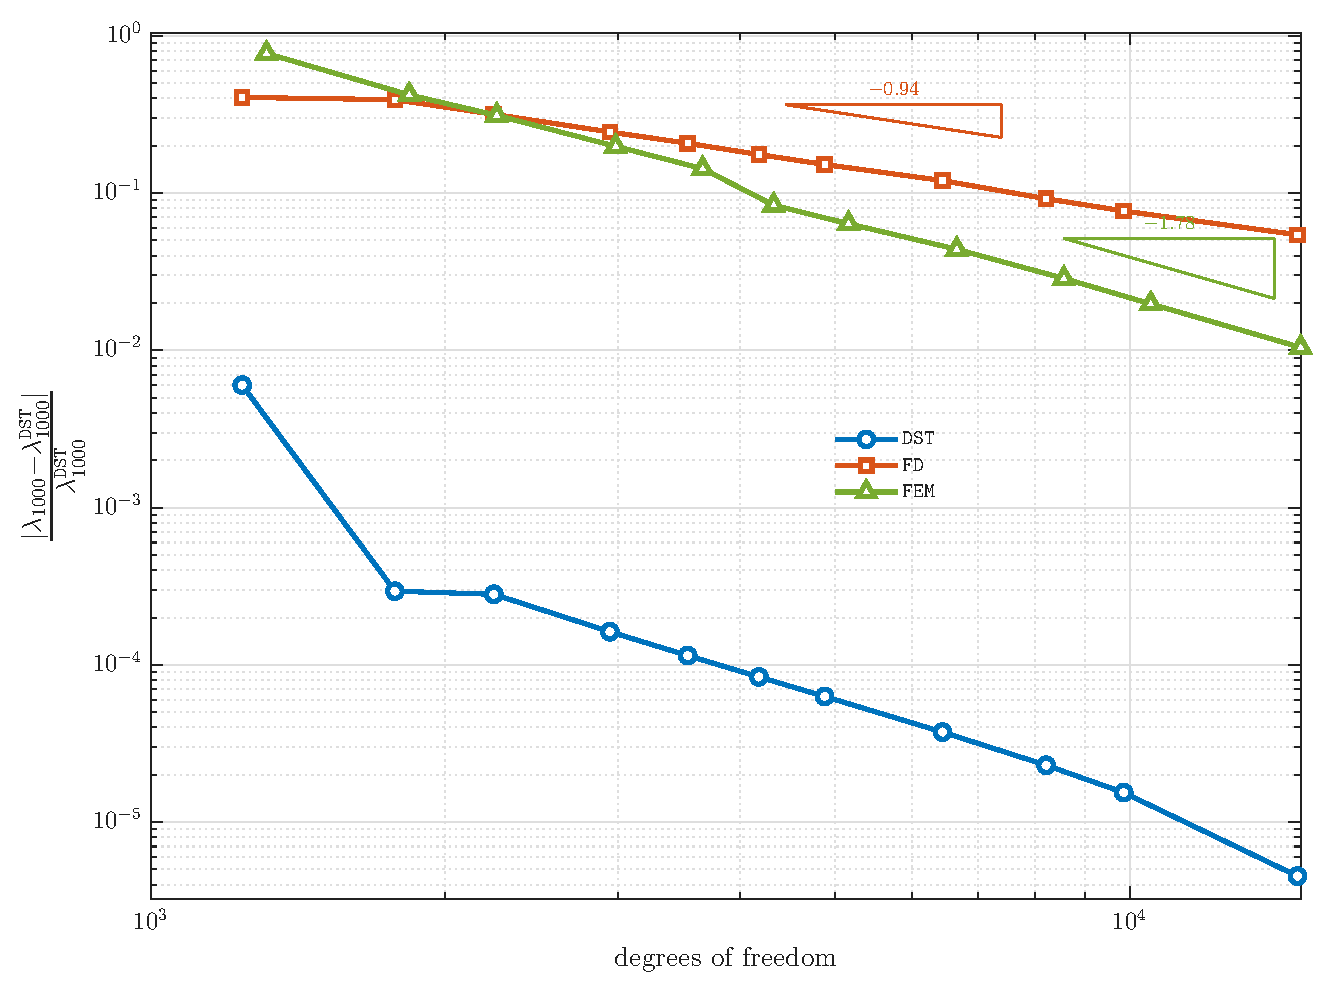
\includegraphics[width=0.45\textwidth]{L_shaped_convergence_lambda1000_error}}
  \caption{The thousandth eigenvalue $\lambda_{1000}$ of Laplace operator, zero Dirichlet boundary conditions, L-shaped domain \texttt{L\_shaped}. Eigenvalue $\lambda_{1000}$ computed by each discretisation \texttt{DST}, \texttt{FD} and \texttt{FEM} with varying degrees of freedom; compared with the reference eigenvalue $\lambda_{1000}^{\text{DST}}$ computed by \texttt{DST} with 14840 degrees of freedom. Resolutions carrying fewer than 1000 degrees of freedom cannot supply the eigenvalue and are left out.}
  \label{fig:convergence_L_shaped_lambda1000}
\end{figure}
